% LuaLaTeX-ja を用いた卒業論文テンプレート（内容更新版）
\documentclass[a4paper,11pt]{ltjsreport}

%======================= パッケージ =======================
\usepackage{luatexja}
\usepackage{amsmath,amssymb}
\usepackage{bm}
\usepackage{graphicx}
\usepackage{ascmac}
\usepackage[top=20mm,bottom=30mm,left=20mm,right=20mm]{geometry}
\usepackage{multirow}
\usepackage{url}
\usepackage{color}
\usepackage{pgfplots}
\pgfplotsset{compat=1.18}
\usepgfplotslibrary{groupplots}
\renewcommand{\bibname}{参考文献}

%======================= 本文開始 =========================
\begin{document}

%--------------------- 表紙 ---------------------
\begin{titlepage}
  \centering
  ~~\vspace{1cm}
 
  {\Huge 卒　業　研　究　論　文 \par}
  {\Huge （2025年度）\par}

  \vspace{8cm}

  \begin{tabular}{rl}
    {\LARGE 題　　目}　 & {\LARGE ：低コスト移動ロボットにおける} \\
                         & {\LARGE ~~VLMを用いたターゲット追従の} \\
                         & {\LARGE ~~性能評価} \\ \\ \\
    {\LARGE 指導教員}　 & {\LARGE ：保坂 忠明} \\　 \\ \\
    {\LARGE 学生番号}　 & {\LARGE ：1512221209} \\　 \\ \\
    {\LARGE 氏　　名}　 & {\LARGE ：小坂 尚璃}
  \end{tabular}

  \vfil
  \begin{flushright}
    明治大学理工学部 電気電子生命学科
  \end{flushright}
\end{titlepage}

\tableofcontents

%===========================================================
\chapter{序論}
\label{chap:intro}
\section{研究背景}
近年，画像と言語を同時に扱う基盤モデル（Vision-Language Model, VLM）が普及し，ロボットの行動決定に直接組み込む研究が活発化している。
その研究動向の中心にあるのは，(1) Web 画像やキャプションから学習した一般知識をもとに未知物体や抽象的な指示にも対処できるようにすること，および (2) 環境内の物体やランドマークをクラスラベルなどの意味情報とともに表現した地図を構築し，その上でナビゲーションを行うことである。
これらのアプローチでは，多様なセンサ情報と高い計算資源を前提とし，豊富な事前学習知識を活かした柔軟なナビゲーション性能が報告されている。
一方，教育・ホビー用途や簡易な現場計測のために用いられる低コスト移動ロボットでは，専用 GPU や高精度センサを搭載することは現実的でない。このような場面では，Raspberry Pi 等の小型コンピュータと単一カメラのみを搭載した機体から画像を取得し，外部 PC やクラウド上の VLM に推論をオフロードして進行方向を決定する構成が有力な選択肢となる。地図を作成・保持・参照せず，単一フレーム画像から直接「次の行動」を決めるため，セットアップが短時間で済み，環境変更時のリセット負荷も小さいという利点がある。
しかし，このような地図非依存・単眼カメラ依存の構成では，視覚ノイズや照度変化により判断が乱れやすく，VLM 推論に数秒以上を要する場合には遅延中に機体が進み過ぎる問題が生じる。高機能な VLM を用いても，この種の構成でどの程度安定した追従動作が得られるか，照度や初期位置ずれ，推論遅延が走行安定性にどのような影響を与えるかについては，体系的な実験報告が十分とはいえない。
低コスト移動ロボットにとっては，このシンプルな構成が現実的な選択肢であり，その性能限界と典型的な失敗パターンを実走行で把握することは，教育・プロトタイピングにおける VLM 活用の実装指針として重要である。

\section{先行研究と課題}
本節では，VLM を用いたロボット制御に関する先行研究を概観し，本研究との相違点と課題を整理する。

近年の代表的な研究として，RT-2\cite{rt2} および VL-Maps\cite{vlmaps} が挙げられる。RT-2 は，Web 上の画像およびテキストで事前学習したモデルをロボットデータで追加学習し，カメラ画像とテキスト指示を入力として，ロボットアームが「どの物体を，どの順番で，どのように動かすか」といった操作手順を直接出力する手法である。これにより，未知物体や多様な表現を含む指示に対しても，把持や配置といった操作をゼロショットで生成可能であることが示されている。ただし，GPU を搭載した計算機および高精度センサを備えたロボットプラットフォームを前提としている。

VL-Maps は，移動ロボットが走行中に取得したカメラ画像から，「どこに」「何が」存在するかという意味情報を環境地図上に逐次書き込むことで，意味ラベル付き地図を構築する手法である。利用者が「椅子の近く」「ソファとテレビのあいだ」などの文章で目的地を指定すると，この地図を検索して適切な位置を推定し，そこまでの経路を計画する。あらかじめ物体位置を教えなくても言語による柔軟な目的地指定が可能である一方，地図の構築と検索には高い計算能力とメモリ資源を要する。

これらのアプローチは，未知物体や新しい言い回しにも対応できる汎用性を有するが，いずれも GPU 搭載マシンや複数センサを備えた高価なロボットを前提としており，教育・ホビー用途の低価格ロボットにそのまま適用することは難しい。

これに対して本研究は，低価格の移動ロボットを対象とし，搭載計算資源やセンサ構成が大きく制約された環境を想定する。そのため，単眼カメラで撮影した画像を外部 PC 上の VLM に送信し，得られた出力から「前進」「左」「右」といった単純なコマンドを生成してロボットを制御する，地図非依存の簡潔な構成を採用する。

この構成には，部品コストや準備時間を抑えられるという利点がある一方で，いくつかの問題が想定される。第一に，VLM の推論に数秒を要する場合，その間もロボットは走行を続けるため，指令と実際の位置のずれが生じやすい。第二に，照明条件やカメラの揺れによって画像が変化すると，VLM の出力が不安定になり，ターゲット追従が破綻する可能性がある。第三に，初期位置がわずかに異なるだけでも，遅延や認識誤りが累積し，軌道の分岐を引き起こすことが考えられる。

高性能ロボットを前提とする先行研究では，これらの要因は主たる検討対象とはなってこなかった。しかし，低コスト移動ロボットで VLM を実用的に活用するためには，上記のような要因が走行安定性に与える影響を実機実験により定量的に把握することが重要である。本研究はこの点に着目し，単眼カメラと外部 VLM のみを用いた最小構成においてターゲット追従実験を行い，遅延・照度・初期位置ずれが走行結果に与える影響を明らかにすることを目的とする。

\begin{figure}[htbp]
  \centering
  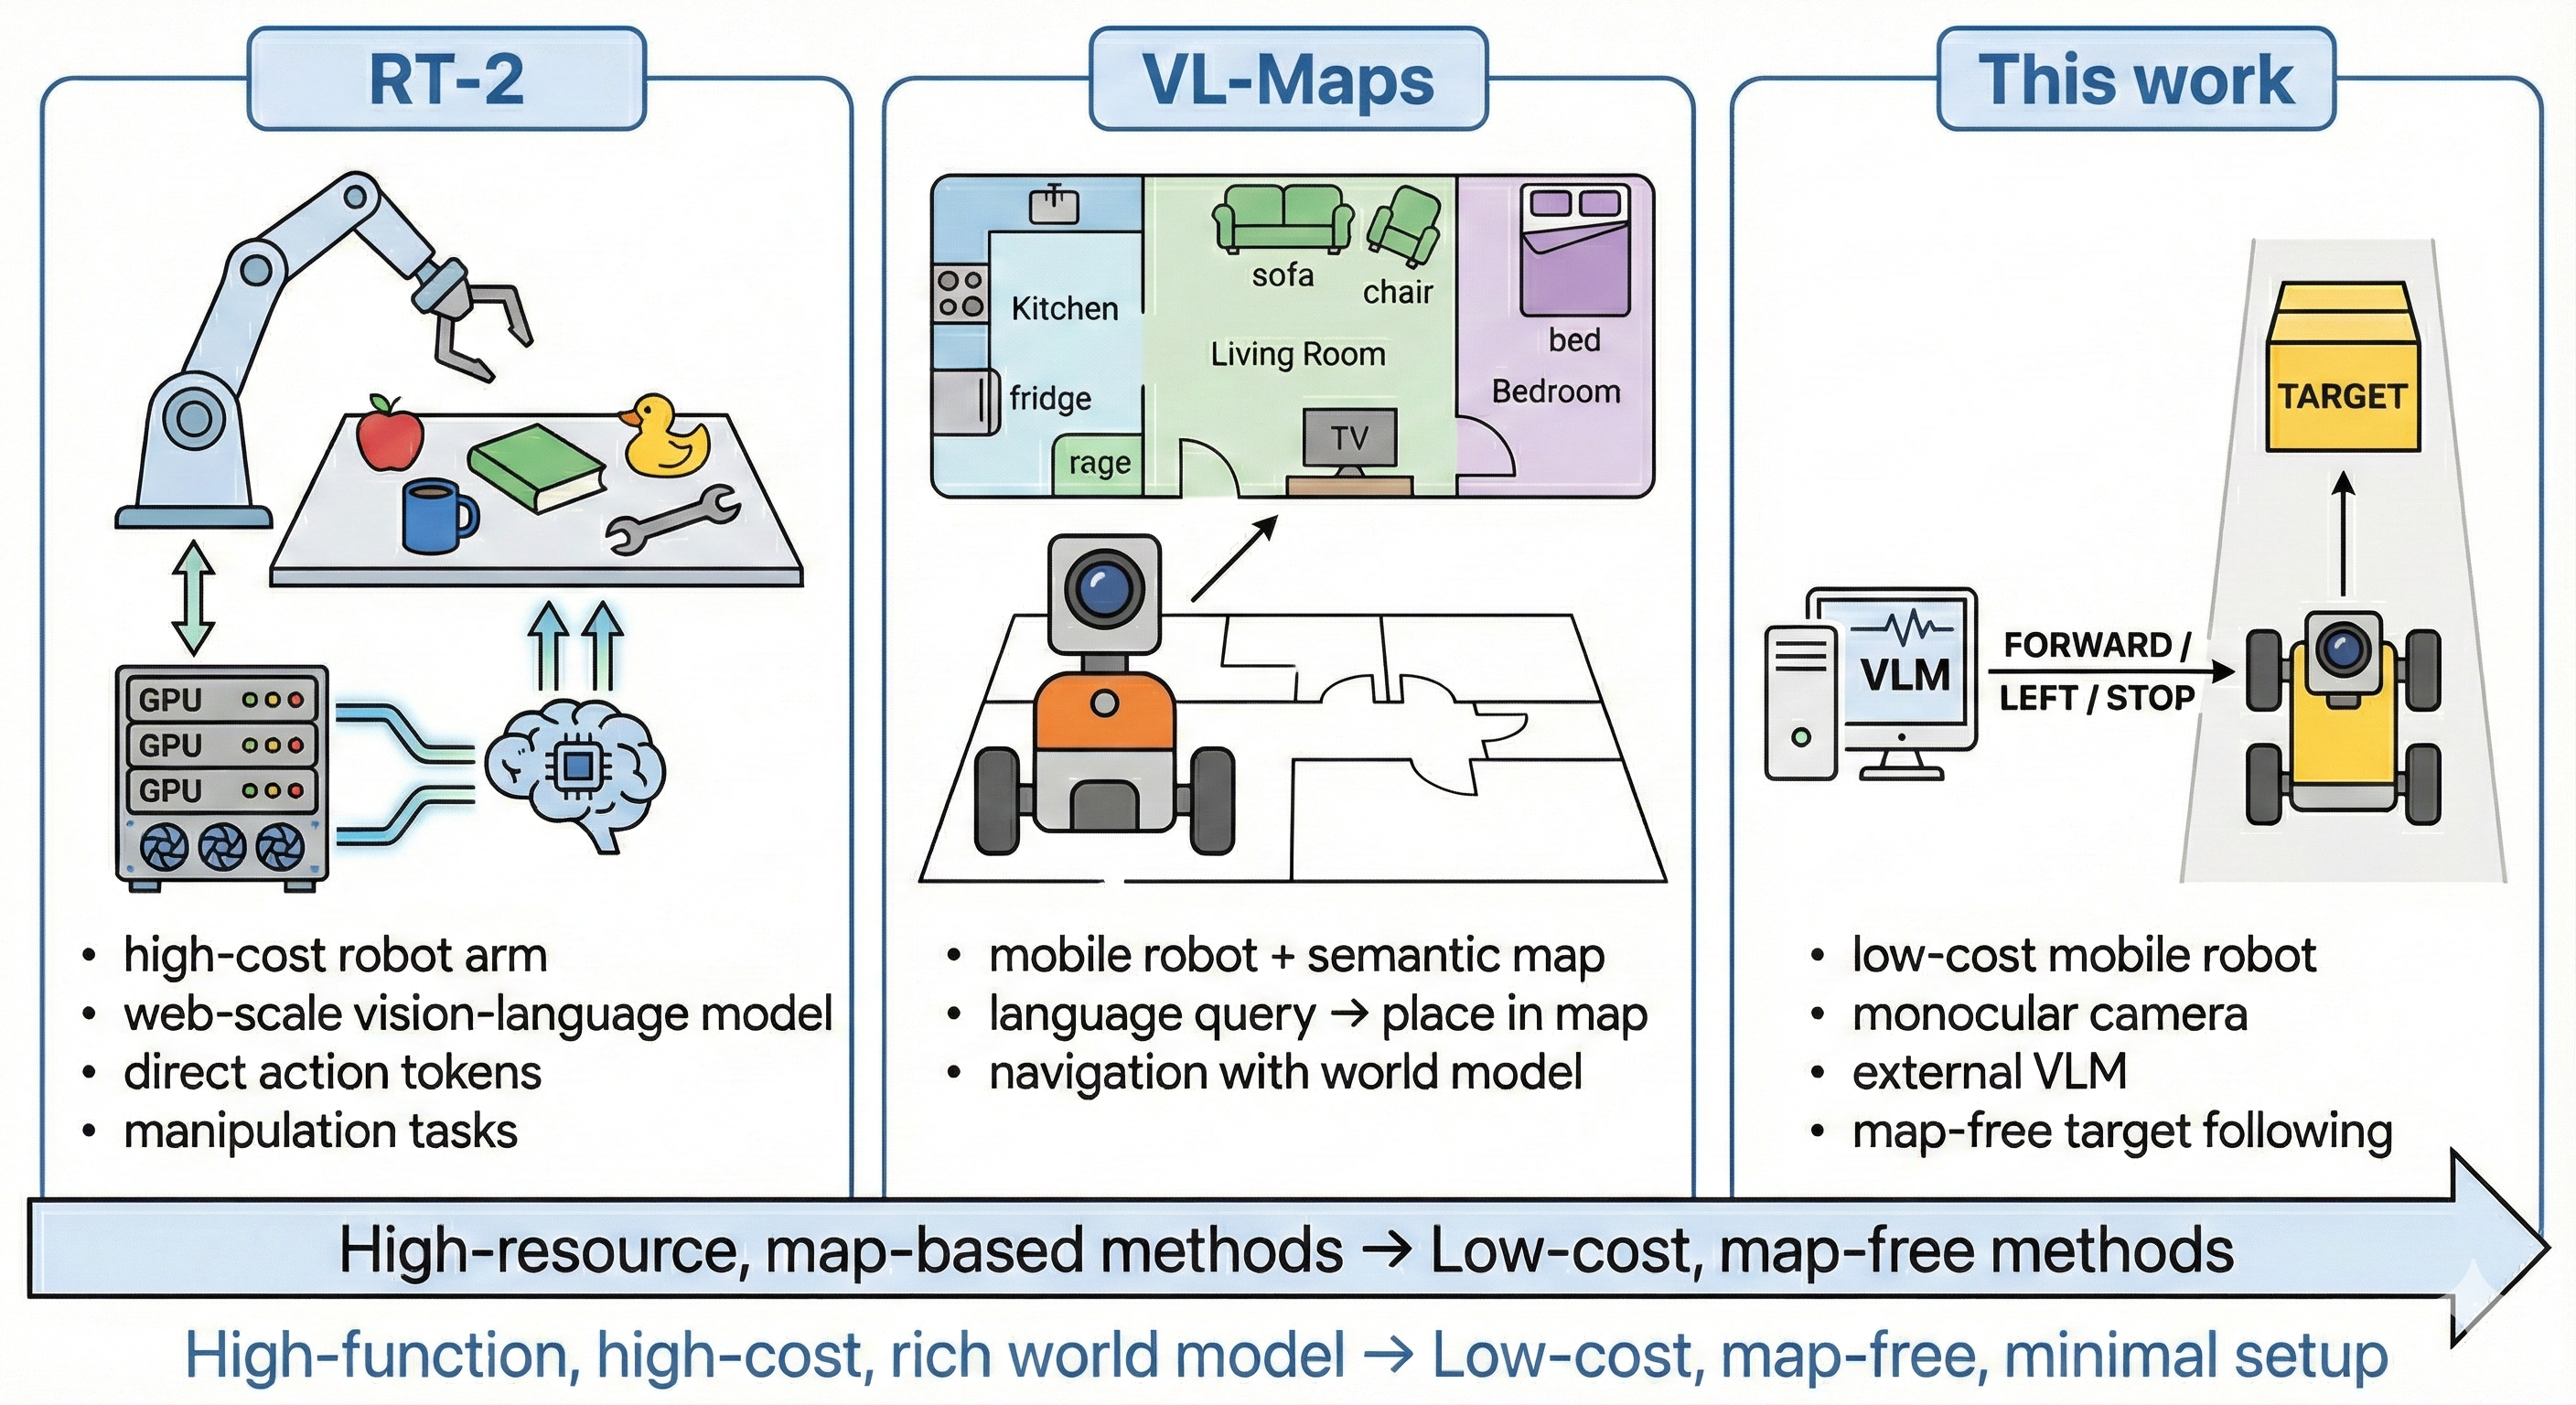
\includegraphics[width=\textwidth]{figs/fig1-1-positioning.png}
  \caption{RT-2・VL-Maps と本研究の位置づけの概念図}
  \label{fig:positioning}
\end{figure}

\section{研究目的}
本研究の目的は，教育・ホビー向けに現実的な「地図なし・単眼カメラ・外部 VLM」構成において，ターゲット追従がどの程度安定して動作しうるかを実走行で評価し，遅延・照度・初期位置ずれが成功率や到達時間，コマンド反転といった走行特性に与える影響を明らかにすることである。
具体的には，OSOYOO 社製 Raspberry Pi Robot Car で取得した画像を PC 側で推論し，視覚判断のみで「黄色いターゲットボックス（以下，ターゲット）に接近し，ターゲットが画像内で十分大きく写った時点で停止する」タスクを遂行させる。明るい環境（照度 873 lx）での走行セットを基準とし，低照度環境（照度 99.9 lx および 23.6 lx）および初期位置ずれ条件での試行を追加する。ログと取得画像から到達可否，所要時間，コマンド反転，推論遅延を取得し，教育・プロトタイピングで再現しやすい実験条件と結果の傾向として整理する。
実施範囲が限定されているため，網羅的な定量化には追加実験が必要であり，本稿では実施した条件における走行特性と，観察された範囲での失敗例について報告する。

\section{論文構成}
本論文の構成を示す。第\ref{chap:method}章でハードウェアと制御手順を述べる。第\ref{chap:experiments}章で実験環境と計測項目を説明し，第\ref{chap:results}章で結果を示す。第\ref{chap:discussion}章で考察を行い，第\ref{chap:conclusion}章で結論と今後の課題を述べる。

%===========================================================
\chapter{手法}
\label{chap:method}

\section{ハードウェア構成}
対象機体は OSOYOO社製 Raspberry Pi Robot Car（2023版）である。計算機として Raspberry Pi 5（8GB RAM）を搭載し，広角 USB カメラ，モータドライバ（L298N），ステアリング用サーボから構成する。カメラ解像度は 640×480，フレームレートは 5 fps とし，走行は室内の平坦な床面（長さ約 2.5 m の直線区間）で行う。

\begin{figure}[htbp]
  \centering
  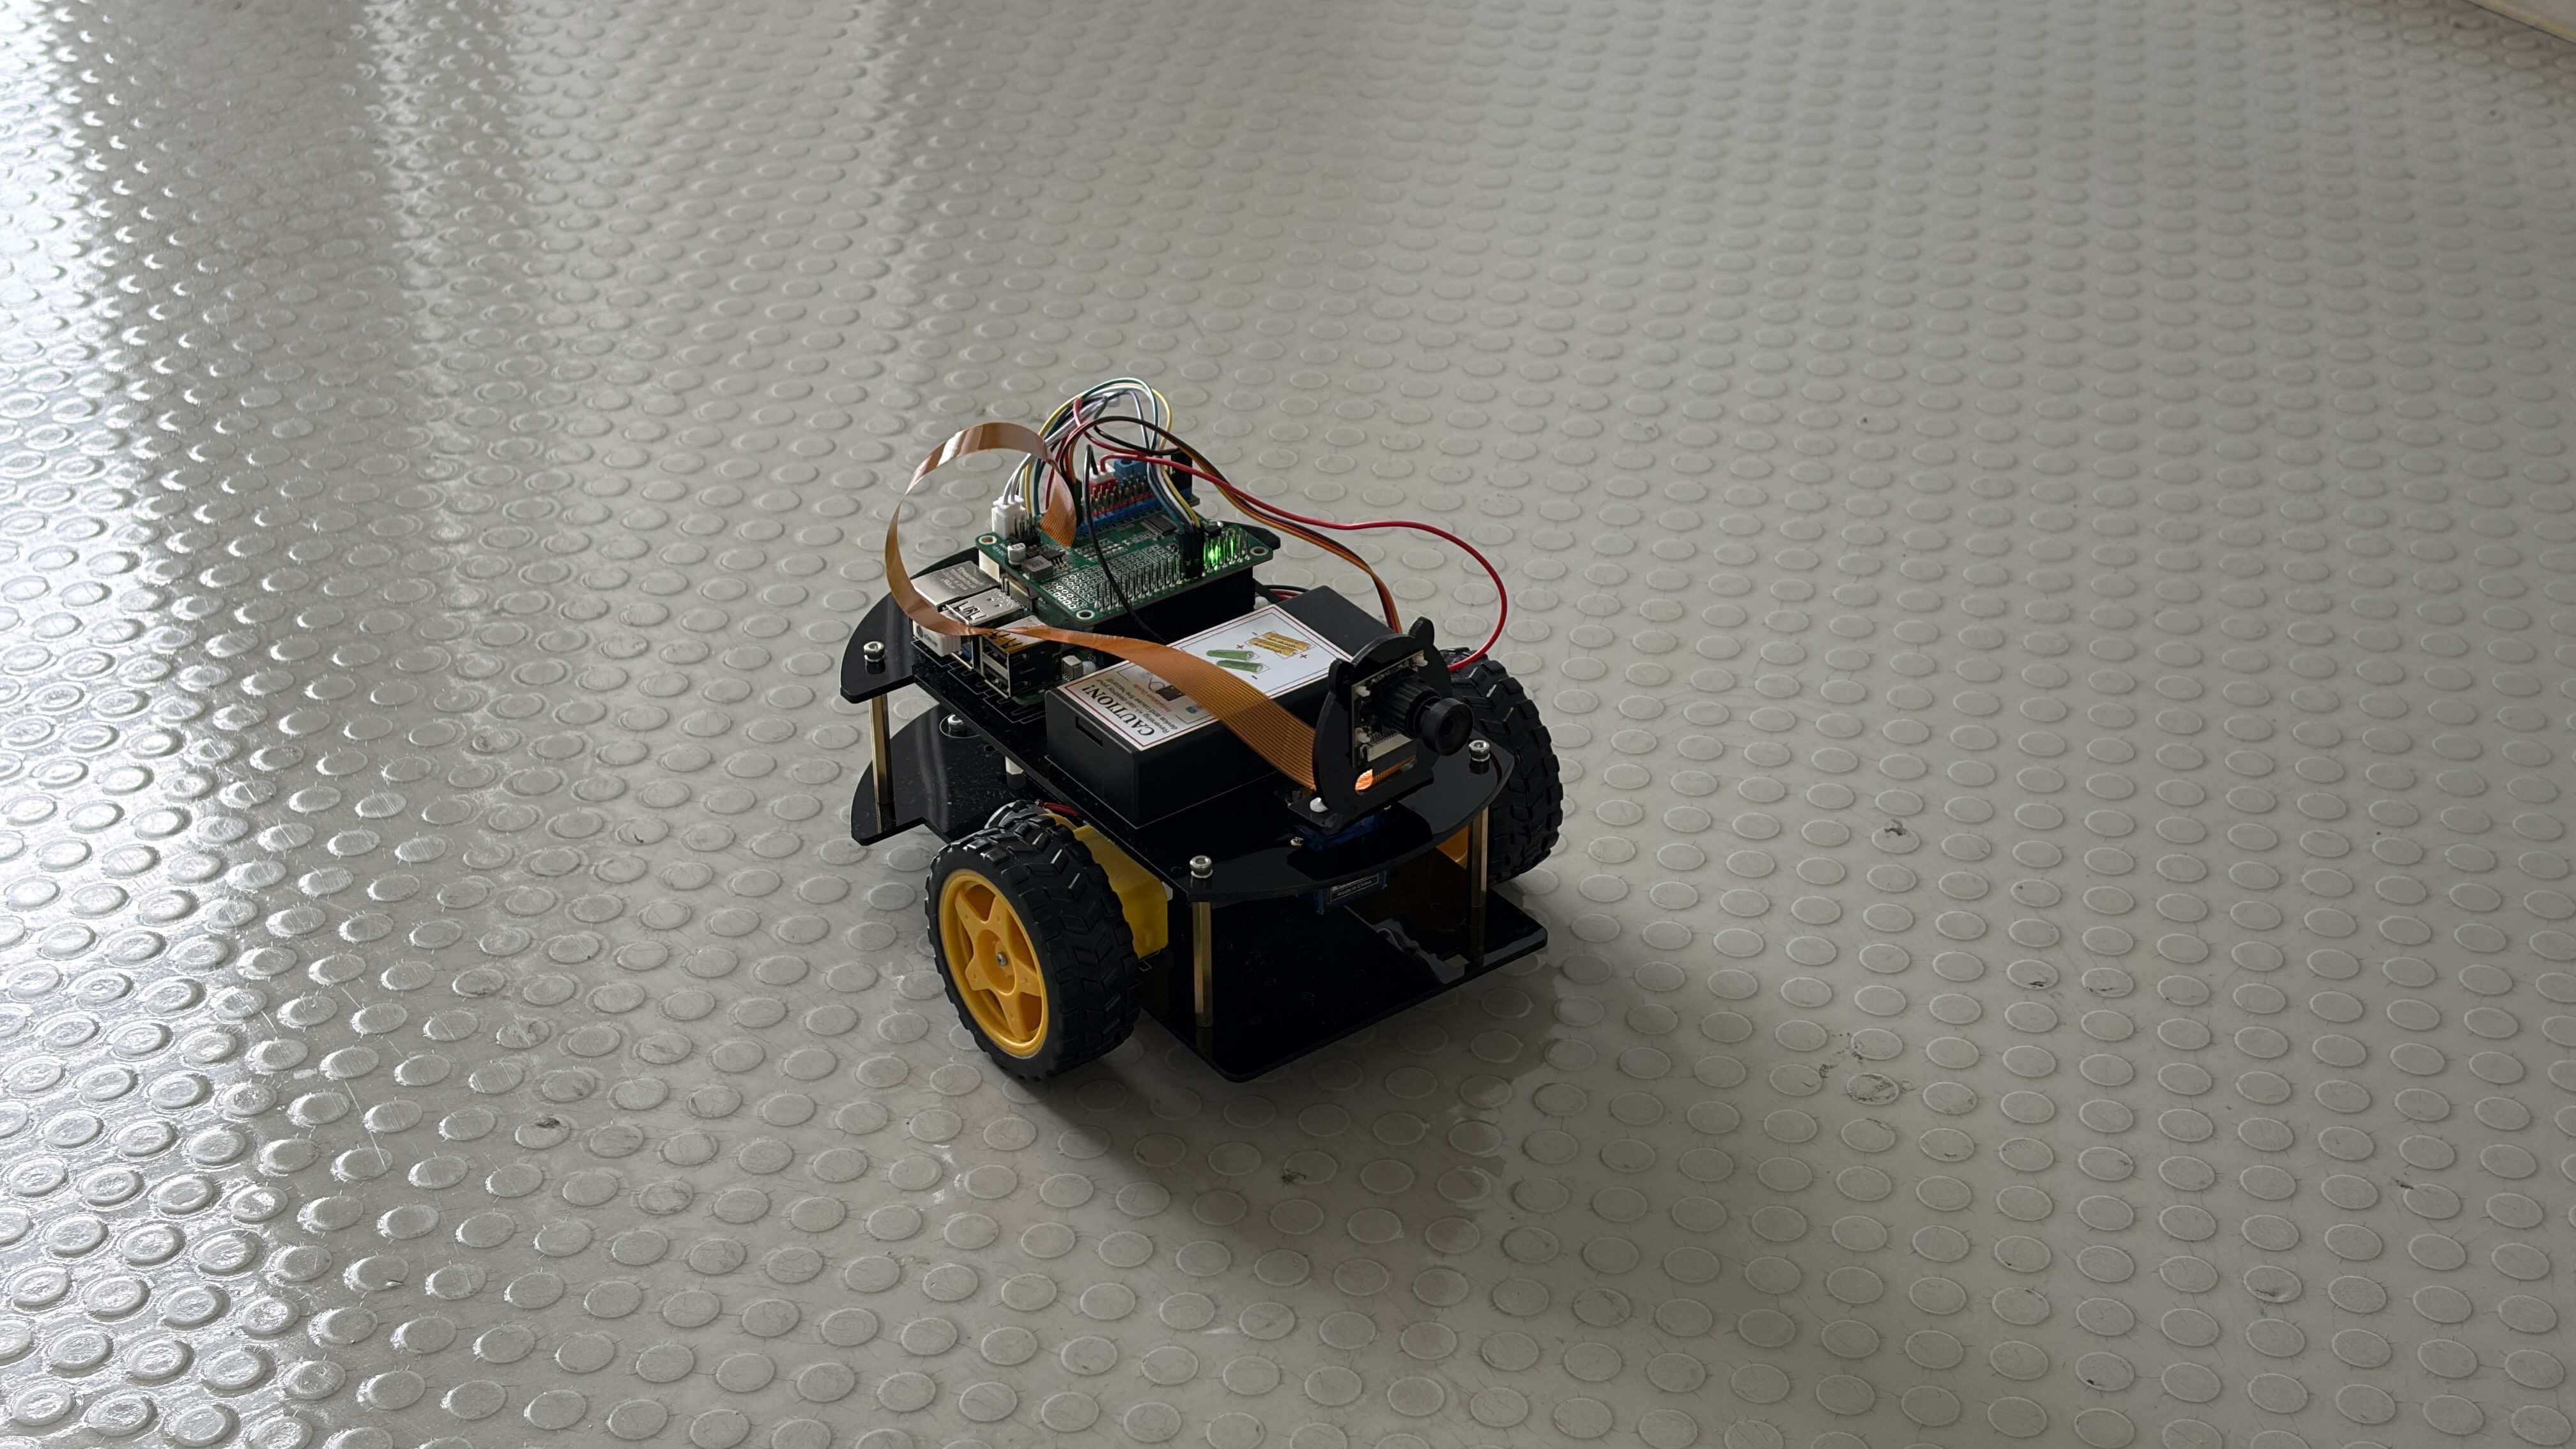
\includegraphics[width=0.9\textwidth]{figs/fig2-1-robot.jpg}
  \caption{実験機体（OSOYOO社製 Raspberry Pi Robot Car）とカメラ搭載位置}
  \label{fig:robot}
\end{figure}

\section{通信とソフトウェア構成}
Raspberry Pi 上では，カメラ画像の取得とモータ・ステアリング制御を行う HTTP サーバ \texttt{raspycar.raspi\_agent} を 8080 番ポートで起動した。サーバは，広角 USB カメラからの 640×480，5 fps の映像から最新フレームを取得し，\texttt{GET /frame.jpg} および \texttt{GET /stream.mjpg} で配信する。また，\texttt{POST /command} に対して \texttt{FORWARD}，\texttt{FORWARD\_SLOW}，\texttt{LEFT}，\texttt{RIGHT}，\texttt{BACK}，\texttt{STOP} のいずれかの文字列を受信すると，内部で左右モータへの速度指令に変換してモータドライバ L298N を駆動する。

PC 側からは同一ネットワーク上の Raspberry Pi に HTTP でアクセスし，\texttt{/frame.jpg} から 10 秒ごとに 1 枚の画像を取得して VLM に入力する。VLM の応答として得られた一語のコマンド（\texttt{FORWARD}，\texttt{FORWARD\_SLOW}，\texttt{LEFT}，\texttt{RIGHT}，\texttt{BACK}，\texttt{STOP} のいずれか）を，そのまま \texttt{/command} に送信してロボットを制御する。推論結果および送信時刻は PC 側でログとして保存し，後の解析に用いる。

\begin{figure}[htbp]
  \centering
  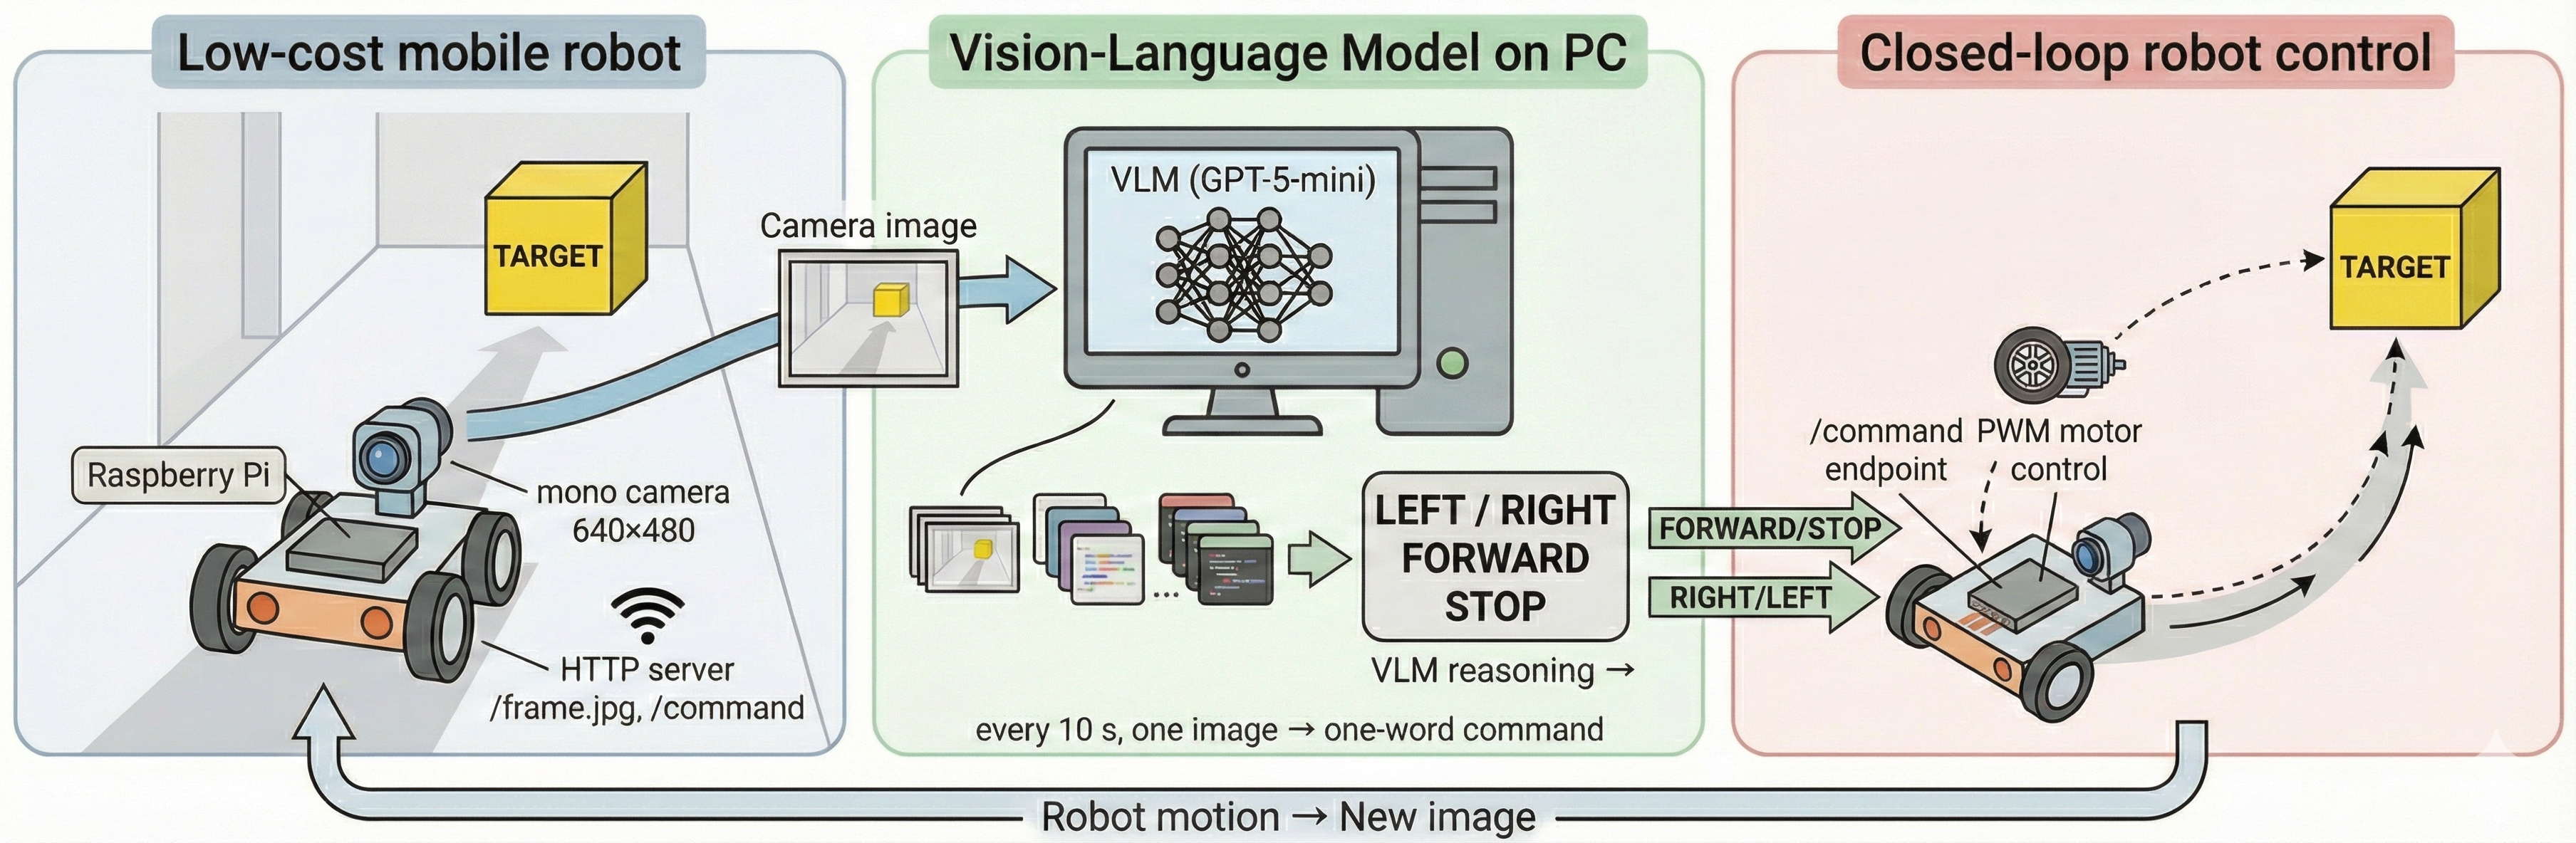
\includegraphics[width=\textwidth]{figs/fig2-2-system.png}
  \caption{提案構成：カメラ画像を外部 VLM で推論し，一語コマンドでロボットを制御するループ}
  \label{fig:system}
\end{figure}

\section{使用モデルとプロンプト}
機体から取得した画像を PC 側で推論する際に使用する VLM として GPT-5-mini-20250807（ローカル実行）を採用する。単一フレームを入力し，プロンプトで以下を明示する。
\begin{itemize}
  \item 黄色いターゲットボックスを画像から検出し，位置と相対距離を判断する。
  \item 応答は \texttt{LEFT}，\texttt{RIGHT}，\texttt{FORWARD}，\texttt{FORWARD\_SLOW}，\texttt{STOP} のいずれか一語に限定する。
  \item 中央付近（画像中央から水平±10\%以内）でターゲットが十分大きい場合は \texttt{STOP}，中央から外れた場合は左右の差分に従って旋回する。
  \item ターゲットが小さいか遠い場合は \texttt{FORWARD}，近づいたら \texttt{FORWARD\_SLOW} で減速する。
  \item ターゲットが視野外または判別不能な場合は \texttt{STOP} とし，前進を避ける。
\end{itemize}
推論に 5--7 秒要するため，ループ間隔は 10 秒とし，各ループで最新フレームを 1 枚取得して命令を更新する。応答は一語のみで，追加説明を含めないようプロンプト内で強制する。

\section{制御手順}
各ループでは，(1) 直近フレームの取得，(2) VLM への送信と一語応答の取得，(3) 応答をそのままモータ指令に変換して送信，(4) 応答と送信時刻のログ化，の順に実行する。ループ間隔は 10 秒とし，各ループで最新フレームを 1 枚取得して命令を更新する。

モータ指令は，正規化された値 $v\in[-1,1]$ を左右ホイールに与え，符号で前進／後退，絶対値で出力の大きさを決める。内部では $\lvert v\rvert$ を PWM デューティ比に変換し，符号に応じてモータドライバ L298N の方向ピンを切り替える。たとえば $v=-0.35$ は「前進方向で約 35\% デューティ」に相当し，$v=-0.14$ であればそのおよそ 40\% の弱い前進となる。

本研究では，前進コマンド \texttt{FORWARD} に対して左右ホイールの目標値をおおよそ $v=-0.35$ 付近に，減速前進 \texttt{FORWARD\_SLOW} に対しては \texttt{slow\_ratio}=0.4 を乗じた $v=-0.14$ 付近に設定した。左右差を付けた \texttt{LEFT}，\texttt{RIGHT} では，片側の出力をわずかに弱めることでアーク状の旋回を実現している。

\texttt{/command} エンドポイントにコマンドを 1 回送信すると，その時点で左右モータの出力が更新され，次のコマンドが届くか，一定時間無通信となってウォッチドッグが作動して \texttt{STOP} に切り替わるまで保持される。したがって，1 回のコマンドで実際に何秒間動くかは，送信間隔とウォッチドッグのタイムアウト設定に依存する。

安全のため，連続して \texttt{STOP} が返った場合はモータを無通電とし，外部操作によってのみ再開できるようにした。

\section{キャリブレーション}
低コスト機体では，モータの個体差やタイヤのネジの締まり具合，床面の摩擦，バッテリ電圧の違いにより，同じ指令を与えても走行量が日ごとに変動しやすい。本研究でも，組み立て誤差を補正するためにステアリングサーボの中立角を \(-68^\circ\) に設定したうえで，左右モータの旋回癖を抑える目的で速度指令に対して \texttt{steer\_offset = 0.01} のオフセット補正を加えたところ，大まかには直進するものの，わずかに左右どちらかへ寄る挙動が残った。

そこで，ロボットを静止状態から単一のモータコマンドを 1 回だけ送信し，その後は追加コマンドを送らずに停止するまで走らせたときの変位を簡易に計測した。座標系は，走行開始時点の機体左上の角を原点とし，機体の横方向を $x$ 軸（右向きを正），縦方向を $y$ 軸（前方を正）とした。この座標系における代表的な変位を表\ref{tab:single_cmd}に示す。

これらの値は，当日の電圧と床面条件における一回計測に基づく近似値であり，指令と変位量の厳密な対応をモデル化したものではない。そのため，本研究ではキャリブレーション結果をあくまで参考情報として扱い，第\ref{chap:results}章で推論遅延と移動距離の関係を議論する際の目安として用いる。

\begin{table}[htbp]
  \centering
  \caption{単一コマンドによる変位（機体左上角を原点とした座標系）}
  \label{tab:single_cmd}
  \begin{tabular}{|c|c|c|c|}
    \hline
    指令 & $\Delta x$ [cm] & $\Delta y$ [cm] & 備考 \\
    \hline
    \texttt{FORWARD} & +1.0 & +31.7 & わずかに右寄りの前進 \\
    \texttt{RIGHT}   & +7.0 & +25.6 & 右方向へのアーク旋回 \\
    \texttt{LEFT}    & $-3.7$ & +27.4 & 左方向へのアーク旋回 \\
    \texttt{BACK}    & +5.2 & $-81.8$ & 後方への後退（前進より距離が大きい） \\
    \hline
  \end{tabular}
\end{table}

%===========================================================
\chapter{実験}
\label{chap:experiments}

\section{環境と照度}
実験は長さ約 2.5 m の室内直線コースで実施した。床は平坦なフロア材で，壁や背景は固定とし，ターゲットは終点に置いた黄色いボックス（“TARGET” と印字）である。初期視野はターゲットが画面中央から水平 $\pm 10\%$，垂直方向は中央よりやや上，サイズは画面比 5--15\% となるように位置決めした。左右ずれ条件では，ターゲット位置を基準の中央配置から右に 68.8 cm，左に 53.0 cm 移動させ，初期視野の水平方向ずれがおおよそ $\pm 20$--$25\%$ となるようにした。

照度はターゲット設置位置に照度計を置いて測定し，明るい条件では 873 lx を維持した。比較のために，99.9 lx および 23.6 lx となるよう照明を落とした低照度条件を二水準用意した。本稿では，これら三水準をそれぞれ 873 lx，99.9 lx，23.6 lx と表記する。

\begin{figure}[htbp]
  \centering
  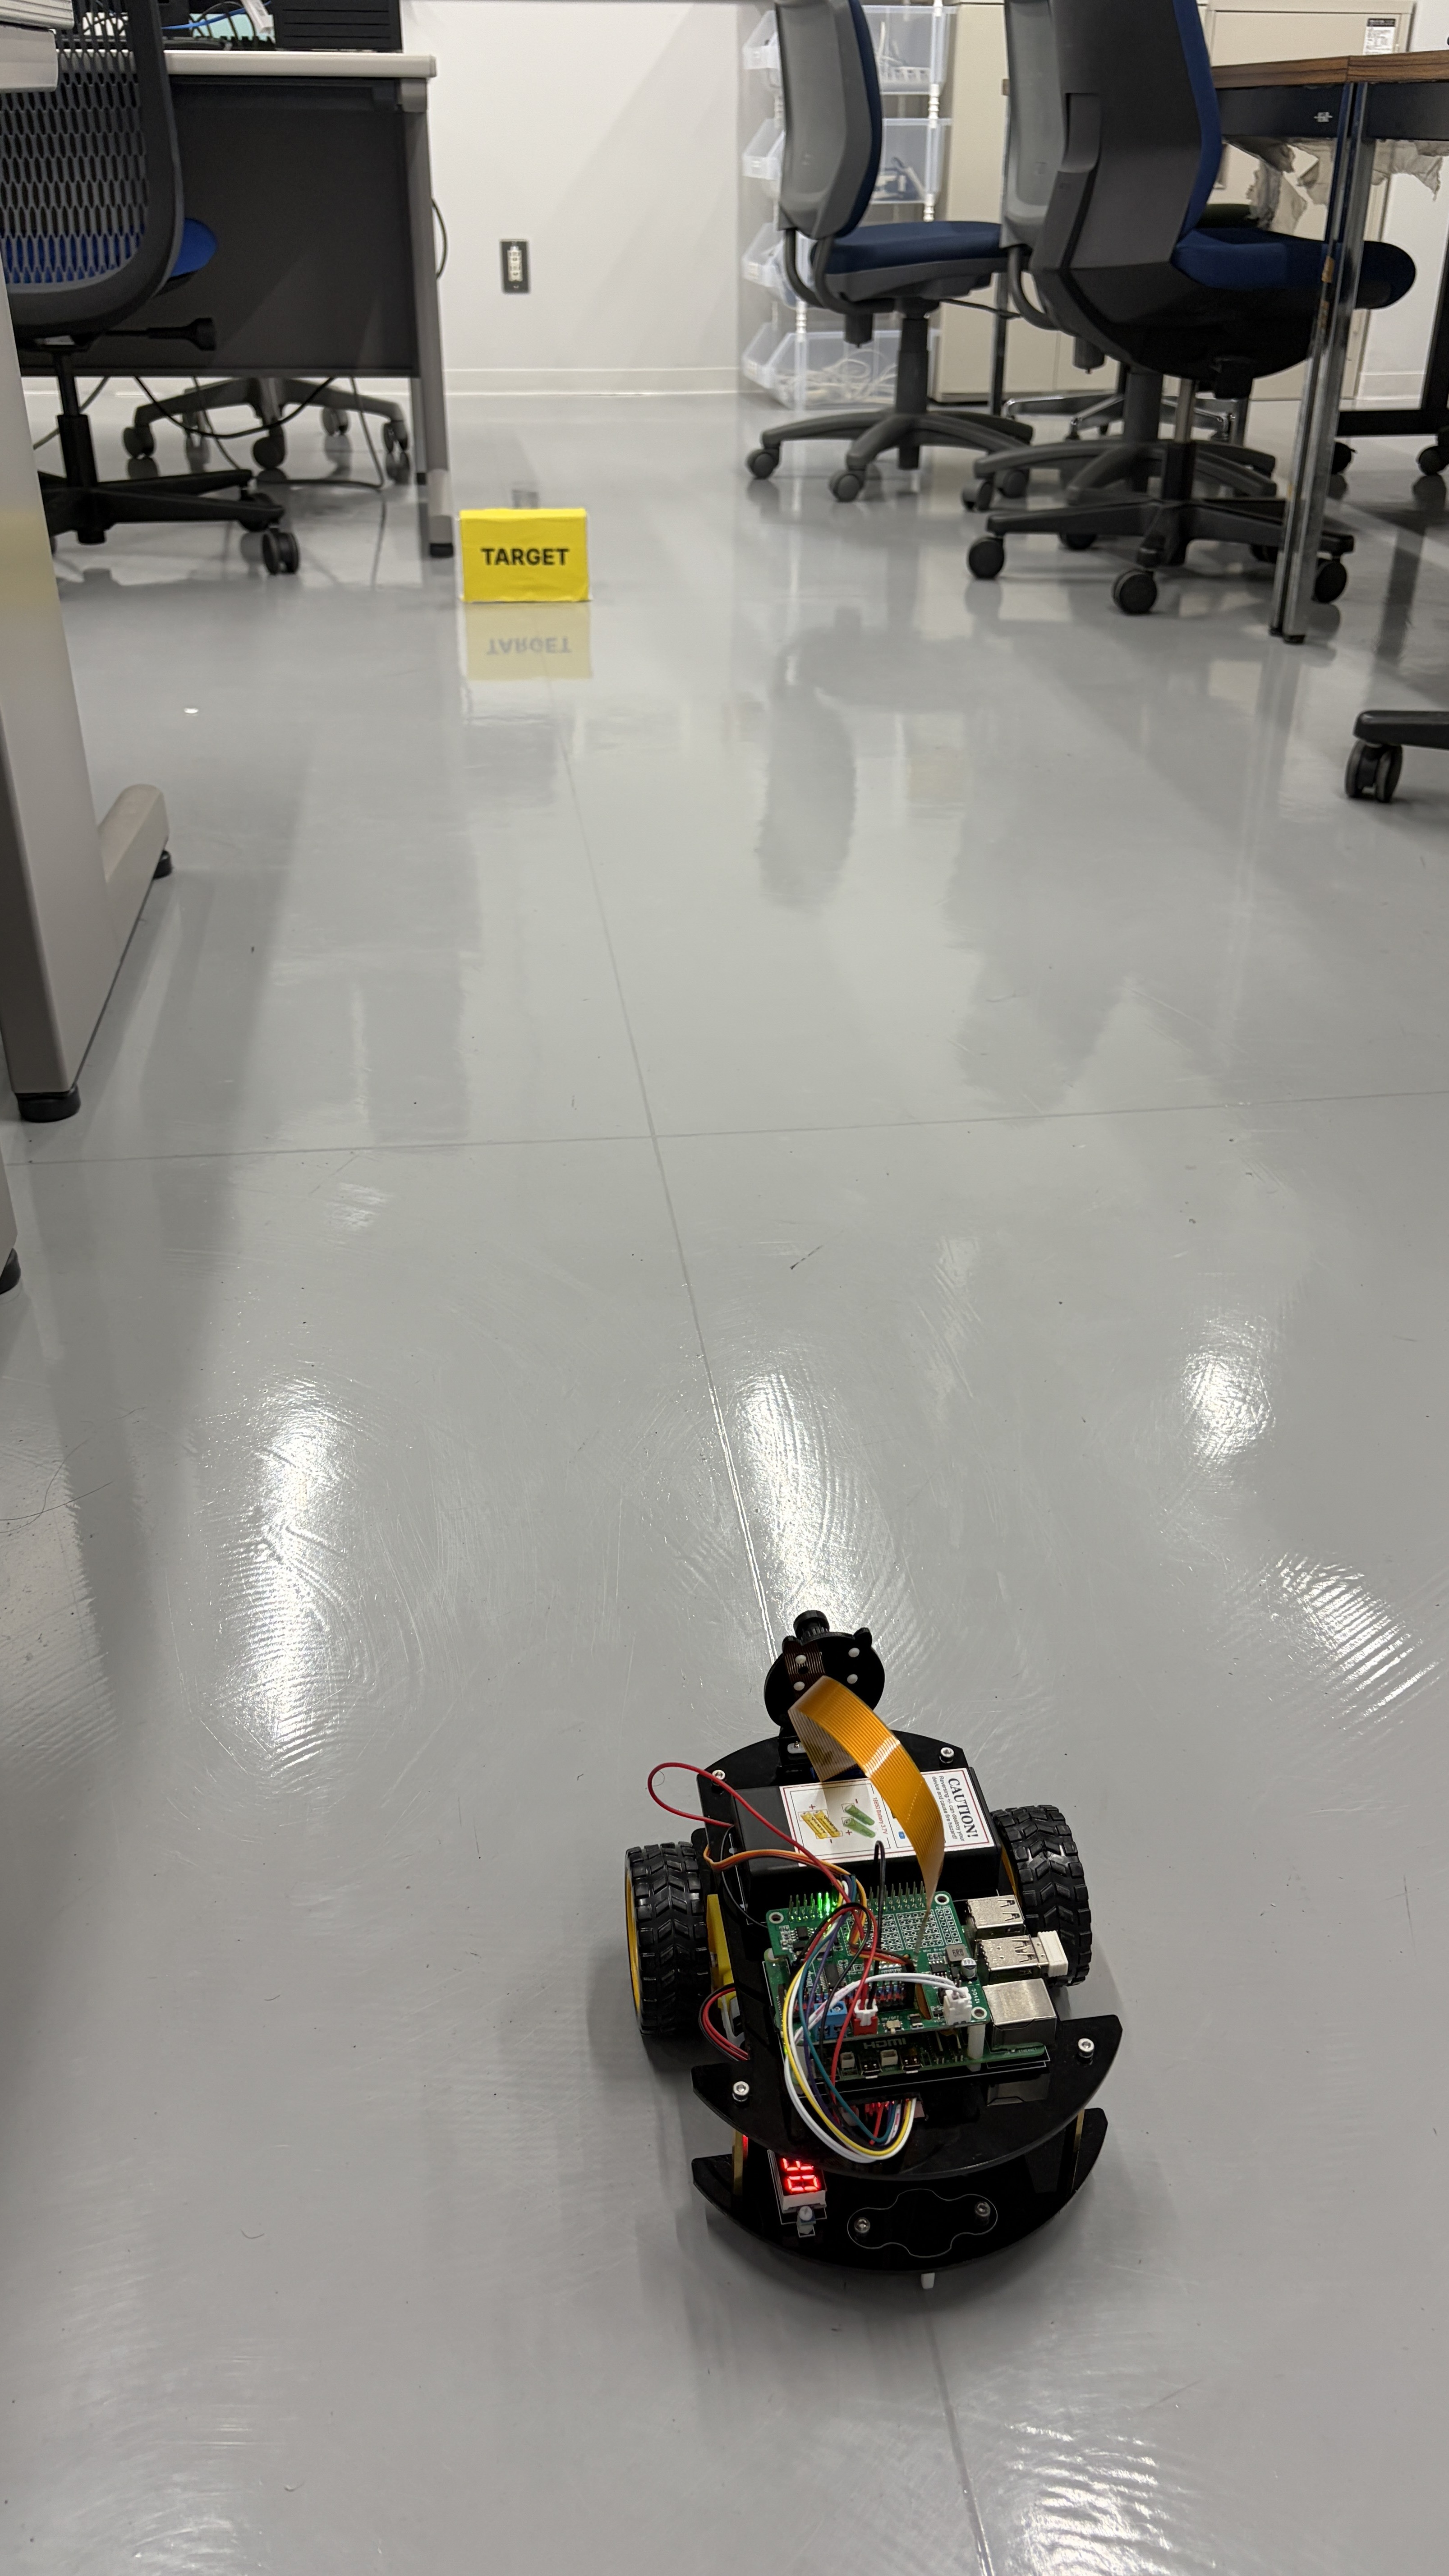
\includegraphics[width=0.58\textwidth]{figs/fig3-1-course.jpg}
  \caption{室内コースとターゲット配置（長さ約 2.5 m，照度はターゲット位置で測定）}
  \label{fig:course}
\end{figure}

\begin{figure}[htbp]
  \centering
  \begin{minipage}[t]{0.32\textwidth}
    \centering
    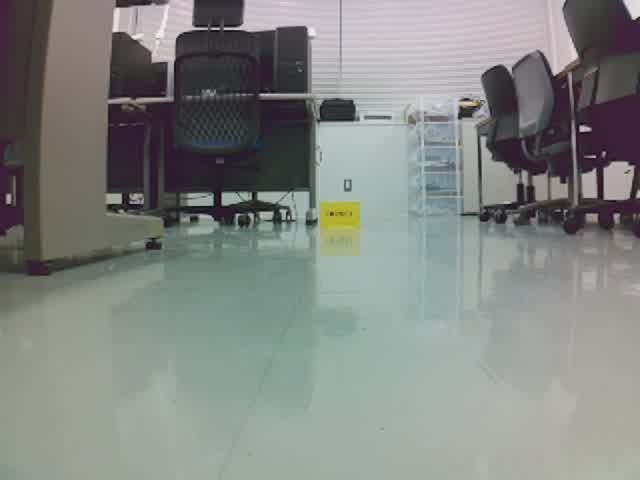
\includegraphics[width=\linewidth]{figs/fig3-2-873lx.jpg}\\[-2mm]
    {\small 873\,lx（明条件・中央配置）}
  \end{minipage}
  \hfill
  \begin{minipage}[t]{0.32\textwidth}
    \centering
    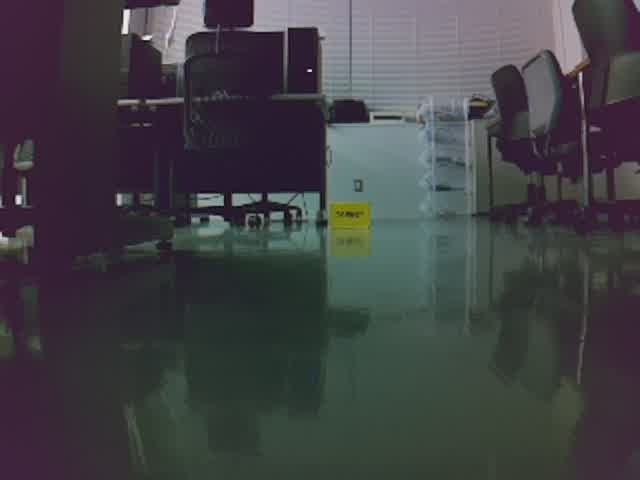
\includegraphics[width=\linewidth]{figs/fig3-2-873lx-offset.jpg}\\[-2mm]
    {\small 873\,lx（明条件・左右ずれ配置）}
  \end{minipage}
  \hfill
  \begin{minipage}[t]{0.32\textwidth}
    \centering
    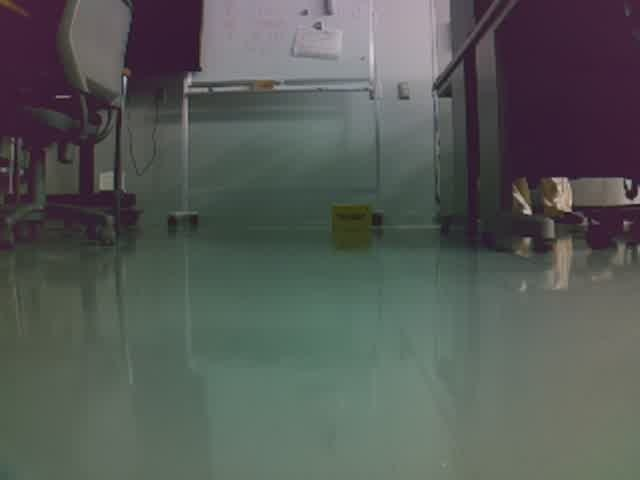
\includegraphics[width=\linewidth]{figs/fig3-2-23lx.jpg}\\[-2mm]
    {\small 23.6\,lx}
  \end{minipage}
  \caption{照度条件別のカメラ画像例（左と中央はいずれも明条件 873\,lx，中央は左右ずれ配置，右は低照度 23.6\,lx）。照度はターゲット位置で測定した。}
  \label{fig:illum_samples}
\end{figure}

\section{試行セット}
実施した走行セットを表\ref{tab:runs}に示す。明条件（873 lx）で中央付近から開始するセットを 6 本，低照度条件を 2 水準（99.9 lx および 23.6 lx）でそれぞれ 2 本，左右ずれ条件を 873 lx で 2 本行った。左右ずれ条件では，3.1節で述べたとおりターゲット位置を中央から右に 68.8 cm，左に 53.0 cm 移動させ，初期視野を水平に 20--25\% ずらした。

各試行では，フレーム画像，VLM 応答，送信コマンド，タイムスタンプ，別カメラで取得した俯瞰画像を保存し，通し番号と照度，開始・終了時刻をメタデータとして付与した。VLM が \texttt{STOP} を 2 回連続で出力し，その時点で機体が静止している場合を「到達」とみなし，その時点で試行を終了した。

\begin{table}[htbp]
  \centering
  \caption{走行セットの構成}
  \label{tab:runs}
  \begin{tabular}{|c|c|c|p{7cm}|}
    \hline
    セット & 本数 & 照度 [lx] & 内容 \\
    \hline
    1 & 6 & 873 & ターゲットが画面中央から水平 $\pm 10\%$，垂直は中央よりやや上，サイズ 5--15\%。基本条件として連続走行し，成功率・到達時間・反転回数・推論遅延を取得。 \\
    2 & 2 & 99.9 & 初期視野はセット1と同一。照度のみ 99.9 lx に下げ，低照度が追従性能に与える影響を確認。 \\
    3 & 2 & 23.6 & 初期視野はセット1と同一。照度を 23.6 lx まで下げ，さらに暗い環境での挙動を確認。 \\
    4 & 2 & 873 & 照度は明条件と同程度。ターゲット位置を中央から右に 68.8 cm，左に 53.0 cm 移動し，初期視野を左右に 20--25\% ずらした条件で耐性を確認。 \\
    \hline
  \end{tabular}
\end{table}

\section{計測項目}
本稿で報告する主な指標は以下のとおりである。
\begin{itemize}
  \item 成功率：ターゲットが画像内で十分大きく写り，VLM が \texttt{STOP} を 2 回連続で出力し，その時点で機体が静止していた試行の割合。
  \item 到達時間：各試行の開始フレームのログ時刻を $t_{\mathrm{start}}$，VLM が \texttt{STOP} を初めて出力したタイミングに対応するフレームのログ時刻を $t_{\mathrm{stop1}}$ とし，到達時間を $t_{\mathrm{stop1}}-t_{\mathrm{start}}$ と定義する。到達時間は成功と判定された試行にのみ与え，失敗試行では未定義とする。
  \item コマンド反転回数：連続する 2 回の指令が前後（\texttt{FORWARD} 系と \texttt{BACK}）または左右（\texttt{LEFT} と \texttt{RIGHT}）で即時反転しているペアの数。各試行で合計し，セットごとに中央値を算出する。
  \item 推論遅延：各コマンドに対する VLM 応答時間をログから取得し，セットごとに中央値と 95 パーセンタイル（95p）を算出する。
\end{itemize}
到達時間と反転回数の中央値は，成功試行に限定して算出し，失敗試行の到達時間は ``--'' として扱う。

%===========================================================
\chapter{結果}
\label{chap:results}
\section{集計結果}
各試行ログから到達可否，VLM 推論結果，送信コマンド列，推論遅延を抽出し，3.3節で定義した指標を条件ごとに集計した結果を表\ref{tab:summary}に示す。各条件の試行本数は 2〜6 本と少ないため，本章では統計的有意差は主張せず，少数試行に基づく傾向として結果を解釈する。

\begin{table}[htbp]
  \centering
  \caption{試行セット別の集計（到達時間・反転中央値は成功試行のみ）}
  \label{tab:summary}
  \begin{tabular}{|c|c|c|c|c|c|c|}
    \hline
    セット & 照度 [lx] & 試行（成功） & 成功率 & 到達時間中央値 [s] & 反転中央値 & 推論遅延中央値 / 95p [s] \\
    \hline
    1 & 873 & 6（4） & 66.7\% & 101 & 0 & 1.10 / 1.61 \\
    2 & 99.9 & 2（1） & 50.0\% & 113 & 0 & 0.87 / 1.30 \\
    3 & 23.6 & 2（1） & 50.0\% & 125 & 2 & 0.80 / 1.25 \\
    4 & 873 & 2（1） & 50.0\% & 124 & 0 & 0.80 / 0.93 \\
    \hline
  \end{tabular}
\end{table}

明条件（873\,lx）のセット1では 6 本中 4 本が成功し，成功率は 66.7\% であった。成功試行の到達時間中央値は 101\,s，反転回数の中央値は 0 回，推論遅延の中央値／95 パーセンタイル（95p）は 1.10／1.61\,s であり，多くのコマンドが 2\,s 未満で応答している。

低照度条件のセット2（99.9\,lx）とセット3（23.6\,lx）はいずれも試行 2 本中 1 本が成功し，成功率 50.0\% となった。成功試行に基づく到達時間中央値はそれぞれ 113\,s，125\,s で，明条件と比べ 10--20\,s 程度長い。反転回数の中央値はセット2で 0 回，より暗いセット3で 2 回であり，低照度ほど前後・左右の揺れが生じやすい傾向が示唆される。推論遅延の中央値／95p は 0.87／1.30\,s および 0.80／1.25\,s であり，照度による大きな差は見られない。

左右ずれ条件のセット4（873\,lx）では試行 2 本中 1 本が成功し，成功率 50.0\% であった。成功試行の到達時間中央値は 124\,s，反転回数中央値は 0 回，推論遅延の中央値／95p は 0.80／0.93\,s となった。照度は明条件と同程度であるが，成功率が 50\% にとどまったことから，初期視野の左右ずれが到達可否や到達時間に影響していると考えられる。

以上より，本実験条件における成功率は 50--66.7\% 程度であり，明条件・中央視野で最も高く，低照度および初期視野ずれの条件では成功率低下と到達時間のわずかな増加がみられた。一方，VLM の推論遅延は全条件でおおむね 1\,s 前後（95p でも 1.6\,s 未満）に収まっており，遅延分布は照度や初期視野の違いによる大きな変動を示さない。

\begin{figure}[htbp]
  \centering
  \begin{tikzpicture}
    \begin{axis}[
      width=0.9\textwidth,
      height=7cm,
      grid=both,
      xmin=0,xmax=30,
      ymin=-20,ymax=290,
      xlabel={$x$ [cm] （右正）},
      ylabel={$y$ [cm] （前方正）},
      legend style={
        font=\scriptsize,
        at={(0.98,0.02)},
        anchor=south east,
        legend columns=3,
        legend cell align=left,
        fill=white,
        draw=none
      },
    ]
      % 成功トライアル（実験セット1, 873 lx）
      \addplot+[color=blue, thick, mark=none] coordinates {
        (0,0)(1.0,31.7)(2.0,63.4)(3.0,95.1)(4.0,126.8)(11.0,152.4)(7.3,179.8)(8.3,211.5)(15.3,237.1)(22.3,262.7)
      }; \addlegendentry{172549（成功）};
      \addplot+[color=green!60!black, thick, mark=none] coordinates {
        (0,0)(1.0,31.7)(2.0,63.4)(9.0,89.0)(10.0,120.7)(11.0,152.4)(18.0,178.0)(19.0,209.7)(20.0,241.4)(27.0,267.0)
      }; \addlegendentry{172908（成功）};
      \addplot+[color=red, thick, mark=none] coordinates {
        (0,0)(1.0,31.7)(2.0,63.4)(9.0,89.0)(10.0,120.7)(11.0,152.4)(18.0,178.0)(19.0,209.7)(15.3,237.1)(11.6,264.5)
      }; \addlegendentry{173222（成功）};
      \addplot+[color=violet, thick, mark=none] coordinates {
        (0,0)(1.0,31.7)(2.0,63.4)(9.0,89.0)(10.0,120.7)(11.0,152.4)(18.0,178.0)(19.0,209.7)(20.0,241.4)(16.3,268.8)
      }; \addlegendentry{173500（成功）};
      \addplot+[color=brown!70!black, thick, mark=none] coordinates {
        (0,0)(1.0,31.7)(2.0,63.4)(9.0,89.0)(10.0,120.7)(11.0,152.4)(12.0,184.1)(19.0,209.7)(20.0,241.4)
      }; \addlegendentry{173846（成功）};
      % 失敗トライアル（破線）
      \addplot+[color=orange, thick, dashed, mark=none] coordinates {
        (0,0)(1.0,31.7)(8.0,57.3)(15.0,82.9)
      }; \addlegendentry{173727（失敗）};

      % 始点と終点マーク
      \addplot+[only marks, mark=o, mark size=2.5pt, color=black] coordinates {
        (0,0)
      };
      \addplot+[only marks, mark=x, mark size=3pt, color=black] coordinates {
        (22.3,262.7) (27.0,267.0) (11.6,264.5) (16.3,268.8) (20.0,241.4) (15.0,82.9)
      };
    \end{axis}
  \end{tikzpicture}
  \caption{セット1（照度 873\,lx）の推定軌跡（コマンド列と表\ref{tab:single_cmd}のキャリブレーション値から積算）。実線は成功試行，破線は失敗試行。}
  \label{fig:trajectory1}
\end{figure}

\begin{figure}[htbp]
  \centering
  \begin{tikzpicture}
    \begin{groupplot}[
      group style={group size=1 by 2, vertical sep=4mm},
      width=0.95\textwidth,
      xmin=0, xmax=115,
      xtick={0,20,40,60,80,100},
      xlabel={経過時間 $t$ [s]},
    ]
    % --- 上段：コマンド系列（階段プロット） ---
    \nextgroupplot[
      height=5.6cm,
      ymin=-1.1, ymax=5.1,
      ytick={-1,0,1,2,3,4,5},
      yticklabels={{STOP},{BACK},{LEFT},{F\_SLOW},{FORWARD},{},{RIGHT}},
      yticklabel style={text width=13mm, align=right},
      xticklabels=\empty,
      xlabel={},
      ylabel={コマンド},
      grid=both,
      legend style={draw=none},
    ]
      % FORWARD=4, RIGHT=5, LEFT=1, STOP=-1, BACK=0, FORWARD_SLOW=2
      \addplot+[const plot, thick, color=blue] coordinates {
        (0,4) (11.487,4) (22.805,4) (34.082,4) (45.348,5) (57.235,1) (68.311,4) (79.492,5) (90.688,5) (102.168,-1) (113.301,-1)
      };
    % --- 下段：推論遅延 ---
    \nextgroupplot[
      height=3.6cm,
      ymin=0, ymax=2.2,
      ytick={0,0.5,1,1.5,2},
      ylabel={推論遅延 [s]},
      grid=both,
    ]
      \addplot+[mark=*, mark size=2.0pt, color=red] coordinates {
        (0,2.713) (11.487,1.449) (22.805,1.283) (34.082,1.239) (45.348,1.229) (57.235,1.844) (68.311,1.034) (79.492,1.141) (90.688,1.061) (102.168,1.447) (113.301,1.083)
      };
    \end{groupplot}
  \end{tikzpicture}
  \caption{セット1（照度 873\,lx）代表試行（ログID: 172549）のコマンド系列と推論遅延。上段は時系列のコマンド（階段プロット），下段は各ループの推論遅延。時間は最初の送信時刻を $t=0$ とする。}
  \label{fig:trajectory2}
\end{figure}

%===========================================================
\chapter{考察}
\label{chap:discussion}
\section{低コスト・地図なし構成の成立性}
本研究の構成は，単眼カメラで取得した画像を外部 PC 上の VLM に送信し，一語コマンドとして返ってきた応答をそのままモータ指令に用いる単純化されたターゲット追従系である。直線コースという単純なタスクであるにもかかわらず，成功率は 50--66.7\% 程度にとどまり，到達時間の中央値も 100\,s 前後と長い。地図やセンサ融合を用いない最小構成では，照度や初期視野のわずかな違いが走行結果に大きく影響し，実用的な信頼性を得るには追加の工夫が必要である。

一方で，GPU 搭載ロボットアームや意味地図を用いる先行研究と比べ，部品コストとセットアップの手間は小さい。12 本という少数試行ながら，ターゲット追従が一定の確率で成立することを実機で確認できた点は，教育用途やプロトタイピングにおける「動く最小例」として意義がある。

\section{推論遅延と移動距離}
推論遅延の中央値は全条件で 0.8--1.1\,s，95p でも 1.6\,s 未満であった。ループ間隔は 10\,s のため，多くのループで開始から数秒以内に応答が得られ，残りの時間は同じコマンドのまま走行する。キャリブレーション（表\ref{tab:single_cmd}）によれば \texttt{FORWARD} 1 回で約 31.7\,cm 前進し，コース長 2.5\,m なら 8 回程度で理論上は到達できる。実際の到達時間中央値は 101--125\,s であり，理想的直進より多くのループを要している。この差分は，停止直前の余分な \texttt{FORWARD} や途中の \texttt{LEFT}/\texttt{RIGHT}/\texttt{FORWARD\_SLOW} など補正コマンドによるものと考えられる。

ログの目視では，ターゲットが十分大きく映っていても最後に \texttt{FORWARD} が選択され通過してしまう失敗が確認できた。単眼画像のみから一語で行動を選ぶ本構成では，STOP への切り替えタイミングを補助する単純なルールの併用が有効と考えられる。

\section{照度および初期視野ずれの影響}
照度を 873\,lx から 99.9\,lx および 23.6\,lx に下げたセット2, 3 では成功率が 50\% に低下し，到達時間中央値も 10--20\,s 伸びた。特に 23.6\,lx では反転回数中央値が 2 回となり，暗所でターゲット輪郭のコントラスト低下により \texttt{LEFT}/\texttt{RIGHT} の揺れが増えた可能性がある。一方，推論遅延分布は条件間で大きく変わらず，失敗の主因は遅延時間よりも低照度下の認識不安定さにあると考えられる。

左右ずれ条件（セット4）は照度が明条件に近いにもかかわらず成功率 50\% にとどまり，到達時間中央値も 124\,s と長かった。初期視野を水平方向に 20--25\% ずらすだけでも，1 回の旋回では中心に戻り切らず，追加の旋回や前進を経て軌道が分岐する試行が確認された。地図を持たない構成では初期条件のわずかな差が VLM の判断と行動列に累積的な影響を与えることが示唆される。

\section{本研究の限界と今後の改善}
本研究の主な制約は試行数の少なさであり，各条件 2--6 本，成功試行 1--4 本では統計的な有意差検定は難しい。直線コースの単純な環境と単一の VLM 構成に基づくため一般性も限定される。

今後の改善候補として，(1) キャリブレーション結果を用いて推論遅延中の移動距離を見積もり，ターゲット近傍では \texttt{FORWARD} を抑制する簡易制御を導入すること，(2) 低照度時にガンマ補正やヒストグラム平坦化などの画像前処理を加えて VLM 入力を安定させること，(3) 初期視野ずれに対して二連続旋回や「中央を通過したら減速する」などの補助規則を導入すること，(4) 試行数と環境の多様性を増やし体系的に評価することが挙げられる。

%===========================================================
\chapter{結論}
\label{chap:conclusion}
本研究では，教育・ホビー用途を想定した低コスト移動ロボットを対象に，地図や複雑なセンサ統合を用いず，単眼カメラと外部 VLM のみでターゲット追従を行う構成を設計し，実走行で性能を評価した。OSOYOO社製 Raspberry Pi Robot Car の画像を PC 側で推論し，一語コマンド（\texttt{FORWARD}/\texttt{LEFT}/\texttt{RIGHT}/\texttt{STOP} など）をそのままモータ指令として用いる制御ループを構成し，照度や初期視野条件を変えた 12 本の走行セットについて，成功率，到達時間，反転回数，推論遅延を指標として整理した。

明条件・中央視野では成功率 66.7\%，到達時間中央値 101\,s 程度で追従が成立した一方，低照度および初期視野ずれでは成功率が 50\% 程度に低下し，到達時間も 10--20\,s 増加した。推論遅延は全条件で中央値 1\,s 前後，95p でも 1.6\,s 未満に収まり，失敗の多くは低照度下の認識不安定さや STOP への切り替え遅れに起因すると考えられる。高価なロボットプラットフォームを前提とする RT-2 や VL-Maps と異なり，低コスト・地図なし構成の現実的な性能と典型的な失敗パターンを実機ベースで示した点に意義がある。

本稿は 12 本の少数試行，単一環境・単一 VLM に基づく探索的知見であり，一般的な性能評価としては不十分である。今後はキャリブレーションと画像前処理を組み込んだ制御則の改善，行動表現やフレーム履歴の活用による STOP タイミング最適化，環境および試行数の拡大を通じて，地図なし・単眼カメラ・外部 VLM 構成の限界と改良余地を体系的に明らかにする必要がある。本研究で示した評価枠組みと初期結果は，そのための基礎データとして位置づけられる。

%===========================================================
\bibliographystyle{junsrt}
\bibliography{mybibfile}

%===========================================================
\end{document}
